%\documentclass[12pt]{article}
%
%\title{Specifikacija programske potpore}
%
%\usepackage[slovene]{babel}
%\usepackage[utf8]{inputenc}
%\usepackage{hyperref}
%
%%Meta data
%\hypersetup{
%unicode=true
%}
%
%\begin{document}
\chapter{Specifikacija programske potpore}

\section{Funkcionalni zahtjevi}
\textbf{Dionici:}
\begin{enumerate}
\item Gost (neprijavljeni korisnik)
\item Prijavljeni korisnik
\item Dežurni planinar
\item Administrator
\end{enumerate}
\noindent
\textbf{Aktori i njihovi funkcionalni zahtjevi:}
\begin{enumerate}
%\item [\textbf{Aktori i njihovi funkcionalni zahtjevi:}]
\item \underline{Neprijavljeni korisnik (inicijator) može:}
\begin{enumerate}
\item registrirati se ili se prijaviti
%\item pretražiti registrirane korisnike i vidjeti njihove profile %nismo se dogovorili
\item pretražiti i vidjeti unaprijed definirane planinarske izlete
\end{enumerate}

\item \underline{Prijavljeni korisnik (inicijator) može:}
\begin{enumerate}
\item pretražiti registrirane korisnike i vidjeti njihove profile
\item vidjeti i promijeniti svoj profil (sliku, status, bedževe)
\item pretražiti i vidjeti unaprijed definirane planinarske izlete
\item dodati unaprijed definirane planinarske izlete, planinarske domove i skloništa na popis željenih
\item kreirati vlastiti planinarski izlet prema unaprijed definiranom predlošku
\item kreirani planinarski izlet zadržati privatnim ili ga podijeliti sa svim ostalim korisnicima aplikacije
\item ocjenjivati javno dostupne planinarske izlete
\item prijaviti netočne ili neprecizne informacije javno dostupnih planinarskih izleta
\item kreirati događaj vidljiv na zidu obavijesti
\item pozvati korisnike aplikacije s popisa vlastite planinarske zajednice sa zida obavijesti
\item vidjeti popis prihvaćenih ili odbijenih pozivnica
%\item dvosmjerna komunikacija %chat? ili se nismo dogovorili šta je to
\item vidjeti nove objave korisnika s popisa vlastite planinarske zajednice
\item dodati u arhivu ranije odrađene planinarske izlete
\end{enumerate}

\item \underline{Dežurni planinar (inicijator) može:}
\begin{enumerate}
\item pretražiti registrirane korisnike i vidjeti njihove profile
\item vidjeti i promijeniti svoj profil (sliku, status, bedževe)
\item pretražiti i vidjeti unaprijed definirane planinarske izlete
\item dodati unaprijed definirane planinarske izlete, planinarske domove i skloništa na popis željenih
\item kreirati vlastiti planinarski izlet prema unaprijed definiranom predlošku
\item kreirani planinarski izlet zadržati privatnim ili ga podijeliti sa svim ostalim korisnicima aplikacije
\item ocjenjivati javno dostupne planinarske izlete
\item prijaviti netočne ili neprecizne informacije javno dostupnih planinarskih izleta
\item kreirati ili obrisati vlastiti događaj vidljiv na zidu obavijesti
\item pozvati korisnike aplikacije s popisa vlastite planinarske zajednice na postojeći događaj
\item vidjeti popis prihvaćenih ili odbijenih pozivnica
%\item dvosmjerna komunikacija %chat? piše ko fejsbuk
\item vidjeti nove objave korisnika s popisa vlastite planinarske zajednice
\item dodati u arhivu ranije odrađene planinarske izlete
\item dati registriranom korisniku potvrdu o posjetu planinarskog doma
\end{enumerate}

\item \underline{Administrator (inicijator) može:}
\begin{enumerate}
\item vidjeti popis svih registriranih korisnika i njihovih osobnih podataka
\item brisati korisnike i mijenjati im razinu pristupa aplikaciji
\item brisati tuđe događaje
\item promijeniti informacije javno dostupnom planinarskom izletu
\item dodati ili obrisati planinsku rutu
\item dodijeliti ili oduzeti bilo koji bedž registriranim korisnicima
\end{enumerate}

\item \underline{Baza podataka (sudionik):}
\begin{enumerate}
\item pohranjuje sve podatke o korisnicima i njihovim ovlastima
%\item pohranjuje sve podatke o upitima i njihovim rezultatima %nismo se još dogovorili
\end{enumerate}

\end{enumerate}

	\subsection{Obrasci uporabe}
	
		\subsubsection{Opis obrazaca uporabe}
		
			\noindent \underbar{\textbf{UC01 - Registracija}}
			\begin{packed_item}
				
				\item \textbf{Glavni sudionik: } Gost
				\item  \textbf{Cilj:} Izraditi korisnički račun za pristup društvenoj mreži planinara.
				\item  \textbf{Sudionici:} Baza podataka
				\item  \textbf{Preduvjet:} Korisnik u trenutnoj sesiji nije prijavljen.
				\item  \textbf{Opis osnovnog tijeka:}
				
				\item[] \begin{packed_enum}
					
					\item Korisnik odabire opciju za registraciju na ekranu za prijavu.
					\item Sustav otvara ekran za registraciju.
					\item Korisnik unosi ime, prezime, korisničko ime, lozinku i prenosi sliku s uređaja.
					\item Korisnik pritišće gumb za registraciju.
					\item Sustav provjerava točnost podataka.

					\item Baza podataka provjerava da korisnik s tim korisničkim imenom već ne postoji.
					\item Sustav stvara korisnički račun i preusmjerava korisnika na početnu stranicu.
				\end{packed_enum}
				
				\item  \textbf{Opis mogućih odstupanja:}
				
				\item[] \begin{packed_item}
					
					\item[5.a] Podaci su nepotpuni ili pogrešni. 
					\item[] \begin{packed_enum}
						
						\item Sustav daje korisniku do znanja koji podaci su neispravni.
						\item Sustav ide u korak 3.
						
					\end{packed_enum}
					
					\item[6.a] Korisnik s tim korisničkim imenom već postoji. 
					\item[] \begin{packed_enum}
						
						\item Sustav daje korisniku do znanja da mora koristiti drugo korisničko ime.
						\item Sustav ide u korak 3.
						
					\end{packed_enum}
					
				\end{packed_item}
			\end{packed_item}


			\noindent \underbar{\textbf{UC02 - Pregled tuđeg profila}}
			\begin{packed_item}
				
				\item \textbf{Glavni sudionik: } Korisnik
				\item  \textbf{Cilj:} Vidjeti informacije o nekom drugom korisniku planinaru.
				\item  \textbf{Sudionici:} Baza podataka
				\item  \textbf{Preduvjet:} Korisnik je prijavljen. Ne mora biti prijatelj s dotičnom osobom.
				\item  \textbf{Opis osnovnog tijeka:}
				
				\item[] \begin{packed_enum}
					
					\item Korisnik se nalazi na naslovnici (news feed).
					\item Korisnik pretražuje planinara putem tražilice planinara ili pritišće na njegovu sliku, odnosno ime i prezime, tamo gdje se taj planinar već nalazi na naslovnici.
					\item Baza podataka dohvaća podatke o tom planinaru.
					\item Otvara se profil tog planinara.
					
				\end{packed_enum}
				
				\item  \textbf{Opis mogućih odstupanja:}
				
				\item[] \begin{packed_item}
					
					\item[4.a] Korisnik nije prijatelj s dotičnim planinarom. 
					\item[] \begin{packed_enum}
						
						\item Sustav daje korisniku manje informacija o tom planinaru.
					\end{packed_enum}
						
					
				\end{packed_item}
			\end{packed_item}


			\noindent \underbar{\textbf{UC03 - Filtriranje sadržaja naslovnice}}
			\begin{packed_item}
				
				\item \textbf{Glavni sudionik: } Korisnik
				\item  \textbf{Cilj:} Prikazati samo željene planinarske informacije na naslovnici.
				\item  \textbf{Sudionici:} Baza podataka
				\item  \textbf{Preduvjet:} Korisnik je prijavljen i nalazi se na naslovnici.
				\item  \textbf{Opis osnovnog tijeka:}
				
				\item[] \begin{packed_enum}
					
					\item Korisnik se nalazi na naslovnici (news feed).
					\item Odabire opciju filtriranja sadržaja naslovnice.
					\item Odabire opciju filtriranja - slike, događaji, bedževi ili izleti.
					\item Pritišće gumb za filtriranje odabranog sadržaja.
					\item Na naslovnici se prikazuju samo odabrani sadržaji.
					
				\end{packed_enum}
				
				\item  \textbf{Opis mogućih odstupanja:}
				
				\item[] \begin{packed_item}
					
					\item[3.a] Ne postoji niti jedan sadržaj koji zadovoljava filter. 
					\item[] \begin{packed_enum}
						
						\item Sustav obavještava korisnika primjerenom obaviješću.
					\end{packed_enum}
					
					
				\end{packed_item}
			\end{packed_item}
		
		\noindent \underbar{\textbf{UC04 - Prikaz vlastitog profila}}
		\begin{packed_item}
			
			\item \textbf{Glavni sudionik: } Korisnik
			\item  \textbf{Cilj:} Vidjeti vlastite informacije dostupne na ovoj društvenoj planinarskoj mreži.
			\item  \textbf{Sudionici:} Baza podataka
			\item  \textbf{Preduvjet:} Korisnik je prijavljen.
			\item  \textbf{Opis osnovnog tijeka:}
			
			\item[] \begin{packed_enum}
				
				\item Korisnik se nalazi na bilo kojoj kartici (naslovnica, planinarske staze, ...)
				\item Korisnik pritišće na karticu profil.
				\item Baza podataka dohvaća podatke o tom planinaru.
				\item Otvara se vlastiti profil planinara.
				
			\end{packed_enum}
		\end{packed_item}
	
		\noindent \underbar{\textbf{UC05 - Prikaz naslovnice}}
		\begin{packed_item}
			
			\item \textbf{Glavni sudionik: } Korisnik
			\item  \textbf{Cilj:} Vidjeti aktualne informacije i novosti vezane uz prijatelje planinare.
			\item  \textbf{Sudionici:} Baza podataka
			\item  \textbf{Preduvjet:} Korisnik je prijavljen. 
			\item  \textbf{Opis osnovnog tijeka:}
			
			\item[] \begin{packed_enum}
				
				\item Korisnik se nalazi na bilo kojoj kartici u aplikaciji(profil, planinarski izleti, ...).
				\item Pritišće na karticu Naslovnica.
				\item Baza podataka pohvaća podatke o novostima vezanima uz prijatelje dotičnog planinara.
				\item Korisnik pregledava naslovnicu.
				
			\end{packed_enum}
			
			\item  \textbf{Opis mogućih odstupanja:}
			
			\item[] \begin{packed_item}
				
				\item[3.a] Korisnik nema prijatelja. 
				\item[] \begin{packed_enum}
					
					\item Sustav to daje korisniku do znanja te ga potiče da uspostavi neka prijateljstva.
				\end{packed_enum}
			
				\item[3.b] Korisnik ima prijatelje, ali nitko od njih nije aktivan pa se na naslovnici nema što prikazati. 
				\item[] \begin{packed_enum}
					
					\item Sustav obavještava korisnika da kod njegovih prijatelja nema nikakvih novosti te ga motivira da uspostavi nova prijateljstva.
				\end{packed_enum}
				
				
			\end{packed_item}
		\end{packed_item}
		
		\noindent \underbar{\textbf{UC06 - Dodavanje prijatelja}}
		\begin{packed_item}
			
			\item \textbf{Glavni sudionik: } Korisnik
			\item  \textbf{Cilj:} Povezivanje dvaju korisnika te mogućnost interakcije i pregleda sadržaja koji je vidljiv samo prijateljima.
			\item  \textbf{Sudionici:} Baza podataka
			\item  \textbf{Preduvjet:} Korisnik je prijavljen i nije prijatelj s korisnikom kojeg želi dodati.
			\item  \textbf{Opis osnovnog tijeka:}
			
			\item[] \begin{packed_enum}
				
				\item Korisnik se nalazi na naslovnici (news feed).
					\item Korisnik pretražuje planinara putem tražilice planinara ili pritišće na njegovu sliku odnosno ime i prezime tamo gdje se taj planinar već nalazi na naslovnici.
					\item Baza podataka dohvaća podatke o tom planinaru.
					\item Otvara se profil tog planinara.
					\item Korisnik pritišće gumb za slanje zahtjeva za prijateljstvo.
					\item Planinaru se šalje zahtjev za prijateljstvo od korisnika.
					\item Gumb za slanje zahtjeva za prijateljstvo mijenja izgled i obavještava korisnika da je zahtjev za prijateljstvo poslan.
				
			\end{packed_enum}
			
			\item  \textbf{Opis mogućih odstupanja:}
			
			\item[] \begin{packed_item}
				
				\item[3.a] Planinar je prethodno korisniku poslao zahtjev za prijateljstvom. 
				\item[] \begin{packed_enum}
					
					\item Gumb za slanje zahtjeva za prijateljstvo mijenja se u gumb za prihvaćanje zahtjeva za prijateljstvo.
				\end{packed_enum}
					
			\end{packed_item}
		\end{packed_item}
		
		\noindent \underbar{\textbf{UC07 - Pretraživanje planinara}}
		\begin{packed_item}
			
			\item \textbf{Glavni sudionik: } Korisnik
			\item  \textbf{Cilj:} Pronalazak planinara na zajednici pomoću poznatih informacija.
			\item  \textbf{Sudionici:} Baza podataka
			\item  \textbf{Preduvjet:} Korisnik je prijavljen i nalazi se na kartici "Zajednica".
			\item  \textbf{Opis osnovnog tijeka:}
			
			\item[] \begin{packed_enum}
				
				\item Korisnik se nalazi na kartici "Zajednica".
				\item Korisnik pretražuje planinara putem tražilice planinara.
				\item Podaci uneseni u tražilicu uspoređuju se s podacima iz baze podataka te se pronalaze profili planinara koji se podudaraju s unesenim informacijama.
				\item Korisniku se prikazuju pronađeni planinari.
				
			\end{packed_enum}
			
			\item  \textbf{Opis mogućih odstupanja:}
			
			\item[] \begin{packed_item}
					
					\item[3.a] Ne postoji niti jedan planinar koji zadovoljava unesene podatke za pretraživanje.
					\item[] \begin{packed_enum}
						
						\item Sustav obaviještava korisnika primjerenom obaviješću.
					\end{packed_enum}
				
				
			\end{packed_item}
		\end{packed_item}
		
		\noindent \underbar{\textbf{UC08 - Ocjenjivanje javno dostupnih izleta}}
		\begin{packed_item}
			
			\item \textbf{Glavni sudionik: } Korisnik
			\item  \textbf{Cilj:} Ocjenjivanje izleta kako bi se drugim korisnicima olakšao odabir, a kreatoru izleta dala povratna informacija.
			\item  \textbf{Sudionici:} Baza podataka
			\item  \textbf{Preduvjet:} Korisnik je prijavljen i izlet je javno dostupan.
			\item  \textbf{Opis osnovnog tijeka:}
			
			\item[] \begin{packed_enum}
				
				\item Korisnik se nalazi na kartici planinarskog izleta.
					\item Korisnik pritiskom na zvjezdicu odabire koliko zvjezdica (od 1 do 5) želi dati izletu.
					\item Ocjena izleta ažurira se u bazi podataka.
					\item Korisnik sada umjesto praznih zvjezdica vidi koliko je zvjezdica dao javnom izletu. 
				
			\end{packed_enum}
			
			\item  \textbf{Opis mogućih odstupanja:}
			
			\item[] \begin{packed_item}
					
					\item[3.a] Korisnik je već ocijenio izlet.
					\item[] \begin{packed_enum}
						
						\item Sustav omogućuje korisniku da promijeni svoju ocjenu.
					\end{packed_enum}
				
				
			\end{packed_item}
		\end{packed_item}

		\noindent \underbar{\textbf{UC09 - Kreiranje izleta}}
		\begin{packed_item}
			
			\item \textbf{Glavni sudionik: } Korisnik
			\item  \textbf{Cilj:} Kreirati izlet
			\item  \textbf{Sudionici:} Baza podataka
			\item  \textbf{Preduvjet:} Korisnik je prijavljen i nalazi se na naslovnici ili pregledava izlete ili kreira novi događaj.
			\item  \textbf{Opis osnovnog tijeka:}
			
			\item[] \begin{packed_enum}
				
				\item Korisnik se nalazi na naslovnici (news feed) ili pregledava izlete ili kreira novi događaj.
				\item Korisnik odabire karticu "Kreiraj izlet".
				\item Otvara se stranica na kojoj se nalazi predložak za kreiranje izleta.
				\item Korisnik popunjava predložak.
				\item Korisnik odabire opciju "Kreiraj".
				\item Baza podataka sprema podatke.
				\item Korisnik završava s kreiranjem te je vraćen na prethodnu stranicu s koje je proslijeđen na kreiranje.
				
			\end{packed_enum}
			
			\item  \textbf{Opis mogućih odstupanja:}
			
			\item[] \begin{packed_item}
				
				\item[4.a] Korisnik ispuni predložak, ali ne odabere opciju "Kreiraj". 
				\item[] \begin{packed_enum}
					
					\item Sustav obavještava korisnika primjerenom obaviješću.
				\end{packed_enum}
				
				
			\end{packed_item}
		\end{packed_item}
		
		
		\noindent \underbar{\textbf{UC10 - Dodavanje izleta na popis željenih}}
		\begin{packed_item}
			
			\item \textbf{Glavni sudionik: } Korisnik
			\item  \textbf{Cilj:} Dodati izlet na popis željenih.
			\item  \textbf{Sudionici:} Baza podataka
			\item  \textbf{Preduvjet:} Korisnik je prijavljen.
			\item  \textbf{Opis osnovnog tijeka:}
			
			\item[] \begin{packed_enum}
				
				\item Korisnik pregledava javne planinarske izlete.
				\item Nad željenim izletom korisnik označuje ikonu za dodavanje u favorite.
				\item Baza podataka sprema podatke.
			
			\end{packed_enum}
		\end{packed_item}
		
		
		
		\noindent \underbar{\textbf{UC11 - Prijava netočnih/nepreciznih informacija}}
		\begin{packed_item}
			
			\item \textbf{Glavni sudionik: } Korisnik
			\item  \textbf{Cilj:} Prijaviti netočne/neprecizne informacije.
			\item  \textbf{Sudionici:} Baza podataka, Admin
			\item  \textbf{Preduvjet:} Korisnik je prijavljen.
			\item  \textbf{Opis osnovnog tijeka:}
			
			\item[] \begin{packed_enum}
				
				\item Korisnik pregledava javne planinarske izlete.
				\item Korisnik na izletu odabire opciju "Prijavi".
				\item Otvara se oblačić u koji korisnik piše razlog prijave.
				\item Korisnik odabire opciju "Pošalji prijavu".
				\item Baza podataka sprema podatke.
				\item Prijavu zaprima korisnik koji je napravio izlet ili admin ako je izlet predefiniran.
				
			\end{packed_enum}
			
			\item  \textbf{Opis mogućih odstupanja:}
			
			\item[] \begin{packed_item}
				
				\item[3.a] Korisnik napiše razlog prijave, ali ne odabere opciju "Pošalji prijavu". 
				\item[] \begin{packed_enum}
					
					\item Sustav obavještava korisnika primjerenom obaviješću.
				\end{packed_enum}
				
				
			\end{packed_item}
		\end{packed_item}
		
		
		\noindent \underbar{\textbf{UC12 - Kreiranje događaja}}
		\begin{packed_item}
			
			\item \textbf{Glavni sudionik: } Korisnik
			\item  \textbf{Cilj:} Kreirati događaj.
			\item  \textbf{Sudionici:} Baza podataka
			\item  \textbf{Preduvjet:} Korisnik je prijavljen i nalazi se na naslovnici.
			\item  \textbf{Opis osnovnog tijeka:}
			
			\item[] \begin{packed_enum}
				
				\item Korisnik se nalazi na naslovnici.
				\item Korisnik odabire karticu "Kreiraj događaj".
				\item Otvara se stranica na kojoj se nalazi predložak za kreiranje izleta.
				\item Korisnik popunjava predložak.
				\item Korisnik odabire prijatelje iz liste prijatelja .
				\item Korisnik odabire opciju "Kreiraj".
				\item Baza podataka sprema podatke.
				
			\end{packed_enum}
			
			\item  \textbf{Opis mogućih odstupanja:}
			
			\item[] \begin{packed_item}
				
				\item[4.a] Korisnik ispuni predložak, ali ne odabere opciju "Kreiraj". 
				\item[] \begin{packed_enum}
					
					\item Sustav obavještava korisnika primjerenom obaviješću.
				\end{packed_enum}
			
				\item[5.a] Korisnik nije odabrao niti jednog prijatelja. 
				\item[] \begin{packed_enum}
				
					\item Sustav obavještava korisnika da mora odabrati barem jednog prijatelja.
				\end{packed_enum}
			
				\item[5.b] Korisnik nema prijatelja. 
				\item[] \begin{packed_enum}
				
					\item Sustav to korisniku daje do znanja te ga potiče da uspostavi neka prijateljstva.
				\end{packed_enum}
				
				
			\end{packed_item}
		\end{packed_item}
		
		
		
		\noindent \underbar{\textbf{UC13 - Prihvaćanje/odbijanje događaja}}
		\begin{packed_item}
			
			\item \textbf{Glavni sudionik: } Korisnik
			\item  \textbf{Cilj:} Prihvatiti ili odbiti pozivnicu na događaj.
			\item  \textbf{Sudionici:} Baza podataka
			\item  \textbf{Preduvjet:} Korisnik je prijavljen i pozvan na događaj.
			\item  \textbf{Opis osnovnog tijeka:}
			
			\item[] \begin{packed_enum}
				
				\item Korisnik dobije obavijest da je pozvan na događaj.
				\item Korisnik odabire opciju "Prihvati" ili "Odbij".
				\item Baza podataka sprema podatke.
				\item Korisnik koji je poslao pozivnicu dobiva obavijest o tome je li pozivnica prihvaćena.
				
			\end{packed_enum}
		\end{packed_item}
		
		
		\noindent \underbar{\textbf{UC14 - Prihvaćanje/odbijanje dežurnih planinara}}
		\begin{packed_item}
			
			\item \textbf{Glavni sudionik: } Administrator
			\item  \textbf{Cilj:} Prihvatiti ili odbiti registraciju za dežurnog planinara.
			\item  \textbf{Sudionici:} Baza podataka, Korisnik
			\item  \textbf{Preduvjet:} Korisnik je prijavljen i dodijeljena su mu prava administratora.
			\item  \textbf{Opis osnovnog tijeka:}
			
			\item[] \begin{packed_enum}
				
				\item Administrator dobije obavijest o registraciji.
				\item Administrator otvvara popis registracija.
				\item Odabire opciju "Prihvati" ili "Odbij".
				\item Korisnik dobiva obavijest o tome je li registracija prihvaćena.
				\item Baza podataka sprema podatke.
				
			\end{packed_enum}
		\end{packed_item}
		
		
		
		\noindent \underbar{\textbf{UC15 - Dobivanje bedža}}
		\begin{packed_item}
			
			\item \textbf{Glavni sudionik: } Korisnik
			\item  \textbf{Cilj:} Dobivanje bedža.
			\item  \textbf{Sudionici:} Baza podataka
			\item  \textbf{Preduvjet:} Korisnik je prijavljen i postigao je određeni cilj.
			\item  \textbf{Opis osnovnog tijeka:}
			
			\item[] \begin{packed_enum}
				
				\item Korisnik postiže određeni cilj (Prijeđeni kilometri, nadmorska visina,...).
				\item Korisnik prima obavijest da je dobio bedž.
				\item Baza podataka sprema podatke.
				
			\end{packed_enum}
		\end{packed_item}

				\noindent \underbar{\textbf{UC16 - Objavljivanje bedža}}
		\begin{packed_item}
			
			\item \textbf{Glavni sudionik: } Korisnik
			\item  \textbf{Cilj:} Podijeliti vijest osvojenog bedža s prijateljima.
			\item  \textbf{Sudionici:} Baza podataka	%nisam siguran
			\item  \textbf{Preduvjet:} Korisnik je upravo osvojio bedž.
			\item  \textbf{Opis osnovnog tijeka:}
			
			\item[] \begin{packed_enum}
				
				\item Sustav otvara skočni prozor za objavu bedža.
				\item Korisnik pritišće gumb za objavu bedža.
				\item Sustav prikazuje objavu korisniku i svim prijateljima korisnika.
				
			\end{packed_enum}
			
			\item  \textbf{Opis mogućih odstupanja:}
			
			\item[] \begin{packed_item}
				
				\item[2.a] Korisnik pritišće gumb za odustajanje od objave.
				\item[] \begin{packed_enum}
					
					\item Sustav zatvara skočni prozor.
					
				\end{packed_enum}
				
			\end{packed_item}
		\end{packed_item}
	
	
		\noindent \underbar{\textbf{UC17 - Pregled javno dostupnih izleta}}
		\begin{packed_item}
			
			\item \textbf{Glavni sudionik: } Korisnik i gost
			\item  \textbf{Cilj:} Pregledavanje javno dostupnih izleta.
			\item  \textbf{Sudionici:} Baza podataka
			\item  \textbf{Preduvjet:} Korisnik je prijavljen kao gost ili planinar.
			\item  \textbf{Opis osnovnog tijeka:}
			
			\item[] \begin{packed_enum}
				
				\item Korisnik odabire karticu "Planinarski izleti".
				\item Baza podataka izbacuje sve javno dostupne planinarske izlete.
				\item Korisniku se prikazuju svi javno dostupni planinarski izleti.
				
			\end{packed_enum}
		\end{packed_item}
		
		
		
		\noindent \underbar{\textbf{UC18 - Pretraga javnih planinarskih izleta}}
		\begin{packed_item}
			
			\item \textbf{Glavni sudionik: } Korisnik i gost
			\item  \textbf{Cilj:} Pretraživanje i filtriranje javnih planinarskih izleta.
			\item  \textbf{Sudionici:} Baza podataka
			\item  \textbf{Preduvjet:} Korisnik je prijavljen kao gost ili kao planinar.
			\item  \textbf{Opis osnovnog tijeka:}
			
			\item[] \begin{packed_enum}
				
				\item Korisnik odabire karticu "Planinarski izleti".
				\item Baza podataka izbacuje sve javno dostupne planinarske izlete.
				\item Korisniku se prikazuju svi javno dostupni planinarski izleti.
				\item Korisnik odabire opciju za pretraživanje javnih planinarskih izleta.
				\item Korisni upisuje naziv javnog planinarskog izleta.
				\item Korisnik stavlja određene filtere za sužavanje pretrage.
				\item Baza podataka izbacuje sve javne planinarske izlete koji spadaju pod navedenu kategoriju.
				\item Korisniku se prikazuju svi javno dostupni planinarski izleti sortirani po kriteriju korisnika.
				
			\end{packed_enum}
			
			\item	\textbf{Opis mogućih odstupanja:}
			
			\item[] \begin{packed_item}
				
				\item[8.a] Korisniku se ne prikazuje nijedan planinarski izlet jer nijedan ne spada u navedenu kategoriju.
				\item[] \begin{packed_enum}
					
					\item Korisnik mijenja kriterije ili odustaje od pretrage javnih planinarskih izleta.
				\end{packed_enum}
				
			\end{packed_item}
		\end{packed_item}
		
		
		
		\noindent \underbar{\textbf{UC19 - Prijava u aplikaciju}}
		\begin{packed_item}
			
			\item \textbf{Glavni sudionik: } Korisnik
			\item  \textbf{Cilj:} Pristupanje planinarskom dnevniku s pogodnostima prijavljenog planinara.
			\item  \textbf{Sudionici:} Baza podataka
			\item  \textbf{Preduvjet:} Registracija za planinarski dnevnik.
			\item  \textbf{Opis osnovnog tijeka:}
			
			\item[] \begin{packed_enum}
				
				\item Korisnik unosi svoje korisničko ime i zaporku s kojom se registrirao u zasebne obrazce.
				\item Baza podataka prima podatke koje je unio korisnik.
				\item Baza podataka provjerava točnost podataka.
				\item Baza podataka vraća povratnu informaciju o točnosti unesenih podataka sa strane korisnika.
				\item Korisnik je prijavljen u aplikaciju planinarskog dnevnika s pogodnostima prijavljenog planinara.
				
			\end{packed_enum}
			
			\item	\textbf{Opis mogućih odstupanja:}
			
			\item[] \begin{packed_item}
				
				\item[5.a] Korisnik nije prijavljen te je vraćen na stranicu prijave.
				\item[] \begin{packed_enum}
					
					\item Sustav mu javlja da su mu podaci netočni te da ponovno upiše svoje podatke.
				\end{packed_enum}
				
			\end{packed_item}
		\end{packed_item}
		
		
		
		\noindent \underbar{\textbf{UC20 - Nastavi kao gost}}
		\begin{packed_item}
			
			\item \textbf{Glavni sudionik: } Korisnik
			\item  \textbf{Cilj:} Pristupanje planinarskom dnevniku bez pogodnosti prijavljenog planinara.
			\item  \textbf{Sudionici:} Baza podataka
			\item  \textbf{Preduvjet:} -
			\item  \textbf{Opis osnovnog tijeka:}
			
			\item[] \begin{packed_enum}
				
				\item Od ponuđenih opcija korisnik bira "Nastavi kao gost".
				\item Baza podataka mu daje privremeni nadimak.
				\item Korisnik je prijavljen u aplikaciju planinarskog dnevnika bez pogodnosti prijavljenog planinara.
				
			\end{packed_enum}
		\end{packed_item}
		
		
		
		\noindent \underbar{\textbf{UC21 - Pregled osobnih podataka}}
		\begin{packed_item}
			
			\item \textbf{Glavni sudionik: } Korisnik
			\item  \textbf{Cilj:} Pregled osobnih podataka planinara.
			\item  \textbf{Sudionici:} Baza podataka
			\item  \textbf{Preduvjet:} Korisnik je registriran i prijavljen u aplikaciju planinarskog dnevnika.
			\item  \textbf{Opis osnovnog tijeka:}
			
			\item[] \begin{packed_enum}
				
				\item Korisnik je prijavljen u aplikaciju.
				\item Korisnik odabire opciju "Osobni podaci".
				\item Baza podataka prikuplja informacije o planinaru.
				\item Baza podataka šalje informacije o planinaru.
				\item Korisniku se prikazuju njegovi vlastiti podaci o računu.
				
			\end{packed_enum}
		\end{packed_item}
		
		
		
		\noindent \underbar{\textbf{UC22 - Promjena osobnih podataka}}
		\begin{packed_item}
			
			\item \textbf{Glavni sudionik: } Korisnik
			\item  \textbf{Cilj:} Mijenjanje vlastitih podataka planinara.
			\item  \textbf{Sudionici:} Baza podataka
			\item  \textbf{Preduvjet:} Korisnik je registriran i prijavljen u aplikaciju planinarskog dnevnika.
			\item  \textbf{Opis osnovnog tijeka:}
			
			\item[] \begin{packed_enum}
				
				\item Korisnik je prijavljen u aplikaciju.
				\item Korisnik odabire opciju "Osobni podaci".
				\item Baza podataka prikuplja informacije o planinaru.
				\item Baza podataka šalje informacije o planinaru.
				\item Korisniku se prikazuju njegovi vlastiti podaci o računu.
				\item Korisnik odabire koji od podataka želi promijeniti.
				\item Korisnik unosi promjene.
				\item Baza podataka prima nove podatke.
				\item Korisniku se prikazuju ažurirani vlastiti podaci.
				
			\end{packed_enum}
			
			\item	\textbf{Opis mogućih odstupanja:}
			
			\item[] \begin{packed_item}
				
				\item[9.a] Korisnik je unio nove podatke koji su već zauzeti od strane nekog drugog planinara u sustavu.
				\item[] \begin{packed_enum}
					
					\item Aplikacija ga obavještava o tome.
					\item Korisnik je vraćen na prijašnju stranicu gdje mu je označeno koji se podaci nisu uspjeli ažurirati.
				\end{packed_enum}
				
			\end{packed_item}
		\end{packed_item}
		
		
		
		\noindent \underbar{\textbf{UC23 - Završetak i zapisivanje korisnikova uspjeha}}
		\begin{packed_item}
			
			\item \textbf{Glavni sudionik: } Korisnik i dežurni planinar
			\item  \textbf{Cilj:} Zapisivanje korisnikova uspjeha u završavanju planinarskog izleta.
			\item  \textbf{Sudionici:} Baza podataka
			\item  \textbf{Preduvjet:} Korisnik je registriran, dežurni planinar je registriran i dodijeljena mu je titula dežurnog planinara od strane administratora.
			\item  \textbf{Opis osnovnog tijeka:}
			
			\item[] \begin{packed_enum}
				
				\item Korisnik završetkom svojeg planinarskog izleta dolazi do dežurnog planinara u planinarskom domu.
				\item Korisnik daje svoje podatke dežurnom planinaru koji te podatke sprema u svoju arhivu.
				\item Dežurni planinar ažurira podatke zapisanih korisnika u bazi podataka zapisujući da su odradili planinarski izlet na kojem je on dežuran.
				\item Baza podataka se ažurira
				
			\end{packed_enum}
		\end{packed_item}
		
		
		
		\noindent \underbar{\textbf{UC24 - Registracija dežurnog planinara}}
		\begin{packed_item}
			
			\item \textbf{Glavni sudionik: } Korisnik i administrator
			\item  \textbf{Cilj:} Obavljanje registracije za planinara koji želi dobiti titulu dežurnog planinara za neki planinarski izlet.
			\item  \textbf{Sudionici:} Baza podataka
			\item  \textbf{Preduvjet:} Korisnik je registriran kao planinar, administrator ima privilegije administratora.
			\item  \textbf{Opis osnovnog tijeka:}
			
			\item[] \begin{packed_enum}
				
				\item Obični korisnik aplikacije šalje zahtjev kako bi postao dežurni planinar za određeni planinarski izlet.
				\item Baza podataka prima zahtjev.
				\item Zathjev se prosljeđuje administratoru.
				\item Administrator proučava zahtjev te odlučuje hoće li planinar dobiti titulu dežurnog planinara.
				\item Baza podataka se ažurira.
				\item Planinar dobiva titulu dežurnog planinara te novo korisničko sučelje za obavljanje posla dežurnog planinara.
				
			\end{packed_enum}
			
			\item	\textbf{Opis mogućih odstupanja:}
			
			\item[] \begin{packed_item}
				
				\item[6.a] Planinar je odbijen i ne dobiva titulu dežurnog planinara.
				\item[] \begin{packed_enum}
					
					\item Planinar ponovno šalje zahtjev ili nastavlja koristiti aplikaciju bez titule dežurnog. 
				\end{packed_enum}
				
			\end{packed_item}
		\end{packed_item}
		
		
		
		\noindent \underbar{\textbf{UC25 - Naknadno dodavanje odrađenih izleta}}
		\begin{packed_item}
			
			\item \textbf{Glavni sudionik: } Korisnik 
			\item  \textbf{Cilj:} Naknadno dodati svoje odrađene izlete u arhivu.
			\item  \textbf{Sudionici:} Baza podataka
			\item  \textbf{Preduvjet:} Korisnik je registriran kao planinar, korisnik je prijavljen u sustav.
			\item  \textbf{Opis osnovnog tijeka:}
			
			\item[] \begin{packed_enum}
				
				\item Korisnik odabire opciju "Planinarski izleti".
				\item Korisniku se prikazuju svi javni planinarski izleti.
				\item Korisnik odabire planinarski izlet.
				\item Od ponuđenih opcija (ocjenjivanje izleta, prijava netočnih informacija, itd.) odabire opciju za spremanje izleta u arhivu odrađenih.
				\item Planinarski izlet je označen kao odrađen te je spremljen u korisnikovu arhivu koja je izolirana od ostalih podataka kako se izlet ne bi ubrajao u napredak za korisnikove bedževe.
				
			\end{packed_enum}
		\end{packed_item}
		
		
		
		\noindent \underbar{\textbf{UC26 - Brisanje korisničkog računa}}
		\begin{packed_item}
			
			\item \textbf{Glavni sudionik: } Korisnik 
			\item  \textbf{Cilj:} Brisanje računa korisnika planinarskog dnevnika.
			\item  \textbf{Sudionici:} Baza podataka
			\item  \textbf{Preduvjet:} Korisnik je registriran i prijavljen u aplikaciju planinarskog dnevnika.
			\item  \textbf{Opis osnovnog tijeka:}
			
			\item[] \begin{packed_enum}
				
				\item Korisnik odabire opciju "Osobni podaci".
				\item Korisniku se prikazuju vlastiti podaci u sustavu.
				\item Korisnik odabire opciju "Izbriši moj račun".
				\item Korisnikov račun se briše iz baze podataka.
				\item Korisniku se prikazuje stranica za registraciju i prijavu u aplikaciju planinarskog dnevnika.
				
			\end{packed_enum}
		\end{packed_item}
		
		
		
		\noindent \underbar{\textbf{UC27 - Pregled korisnika}}
		\begin{packed_item}
			
			\item \textbf{Glavni sudionik: } Administrator 
			\item  \textbf{Cilj:} Pregledavanje podataka korisnika aplikacije planinarskog dnevnika.
			\item  \textbf{Sudionici:} Baza podataka
			\item  \textbf{Preduvjet:} Korisnik je registran, prijavljen i ima titulu administratora.
			\item  \textbf{Opis osnovnog tijeka:}
			
			\item[] \begin{packed_enum}
				
				\item Administrator odabire opciju "Pregled korisnika".
				\item Administratoru se prikazuje lista svih registriranih korisnika.
				
			\end{packed_enum}
		\end{packed_item}
		
		
		
		\noindent \underbar{\textbf{UC28 - Brisanje korisnika}}
		\begin{packed_item}
			
			\item \textbf{Glavni sudionik: } Administrator 
			\item  \textbf{Cilj:} Izvanredno brisanje korisnika iz sustava od strane administratora.
			\item  \textbf{Sudionici:} Baza podataka
			\item  \textbf{Preduvjet:} Korisnik je registriran, prijavljen i ima titulu administratora.
			\item  \textbf{Opis osnovnog tijeka:}
			
			\item[] \begin{packed_enum}
				
				\item Administrator odabire opciju "Pregled korisnika".
				\item Administratoru se prikazuje lista svih registriranih korisnika.
				\item Administrator odabire korisnika kojeg želi obrisati.
				\item Podaci o korisniku su izbrisani iz baze podataka.
				
			\end{packed_enum}
		\end{packed_item}
	
	
	
		\noindent \underbar{\textbf{UC29 - Prikaz zajednice}}
		\begin{packed_item}
			
			\item \textbf{Glavni sudionik: } Korisnik 
			\item  \textbf{Cilj:} Prikazivanje kartice "Zajednica".
			\item  \textbf{Sudionici:} Baza podataka
			\item  \textbf{Preduvjet:} Korisnik je registriran i prijavljen.
			\item  \textbf{Opis osnovnog tijeka:}
			
			\item[] \begin{packed_enum}
				
				\item Korisnik odabire opciju "Zajednica".
				\item Baza podataka pregledava sve prijatelje od korisnika.
				\item Korisniku se prikazuje kartica "Zajednica".
				
				
			\end{packed_enum}
		\end{packed_item}
	
	
	
		\noindent \underbar{\textbf{UC30 - Brisanje izleta}}
		\begin{packed_item}
			
			\item \textbf{Glavni sudionik: } Administrator
			\item  \textbf{Cilj:} Brisanje izleta iz baze podataka.
			\item  \textbf{Sudionici:} Baza podataka
			\item  \textbf{Preduvjet:} Korisnik je registriran i prijavljen te ima titulu administratora.
			\item  \textbf{Opis osnovnog tijeka:}
			
			\item[] \begin{packed_enum}
				
				\item Administrator odabire opciju "Planinarski izleti".
				\item Administrator odabire planinarski izlet.
				\item Administrator odabire opciju "Brisanje izleta".
				\item Izlet se briše iz baze podataka.
				
				
			\end{packed_enum}
		\end{packed_item}
	
	
	
		\noindent \underbar{\textbf{UC31 - Promjena izleta}}
		\begin{packed_item}
			
			\item \textbf{Glavni sudionik: } Administrator
			\item  \textbf{Cilj:} Promjena detalja o planinarskom izletu.
			\item  \textbf{Sudionici:} Baza podataka
			\item  \textbf{Preduvjet:} Korisnik je registriran, prijavljen te ima titulu administratora.
			\item  \textbf{Opis osnovnog tijeka:}
			
			\item[] \begin{packed_enum}
				
				\item Administrator odabire opciju "Planinarski izleti".
				\item Administrator odabire planinarski izlet.
				\item Administrator odabire opciju "Promjena izleta".
				\item Administrator unosi podatke koje želi promijeniti.
				\item Baza podataka se ažurira s novim podacima.
				
				
			\end{packed_enum}
		\end{packed_item}
	
	
		
		\subsubsection{Dijagrami obrazaca uporabe}
		
			\begin{figure}[H]
				\centering
				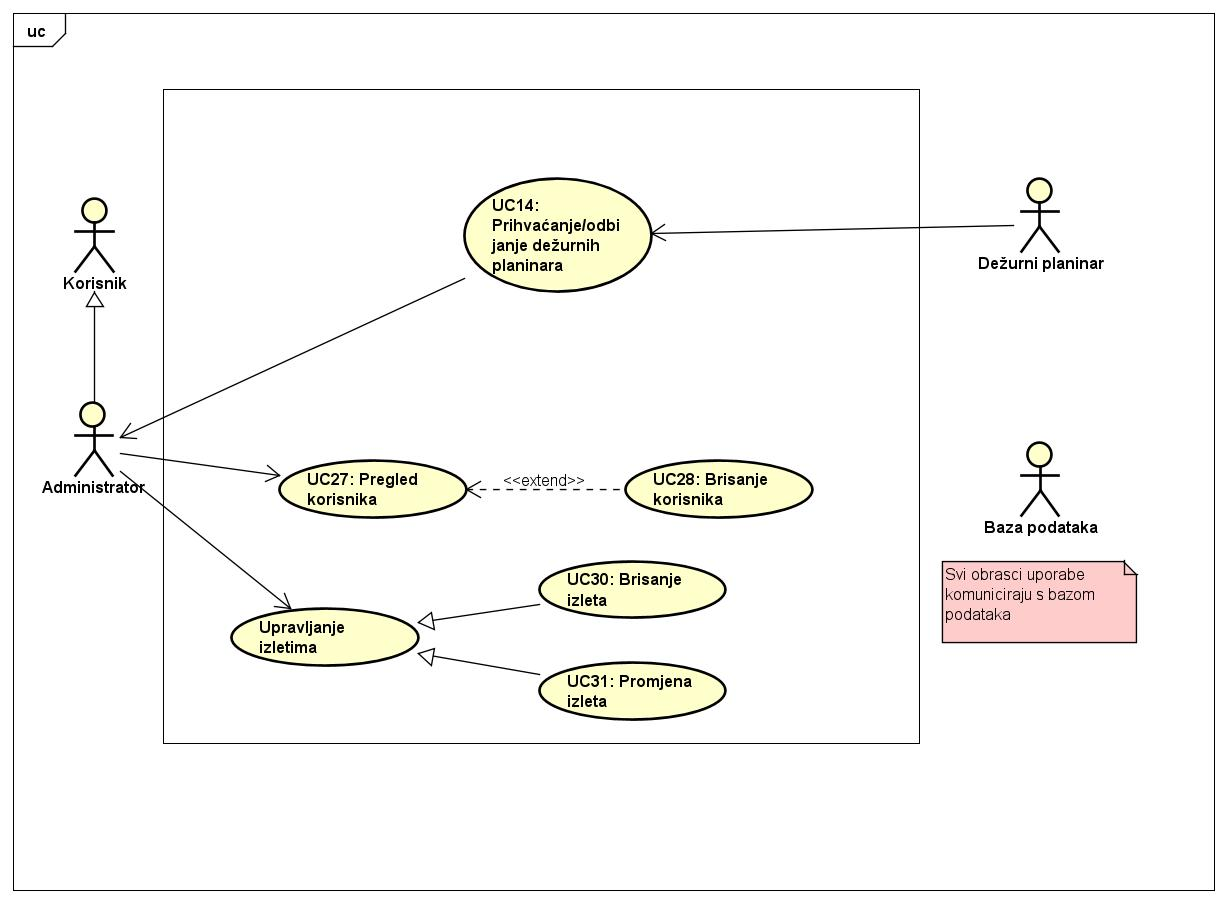
\includegraphics[width=0.9\textwidth]{slike/UC-Administrator.jpg}
				\caption{Dijagram obrasca uporabe, funkcionalnosti administratora}
				\label{fig:mesh1}
			\end{figure}
			
			\vspace{10mm}
			
			\begin{figure}[H]
				\centering
				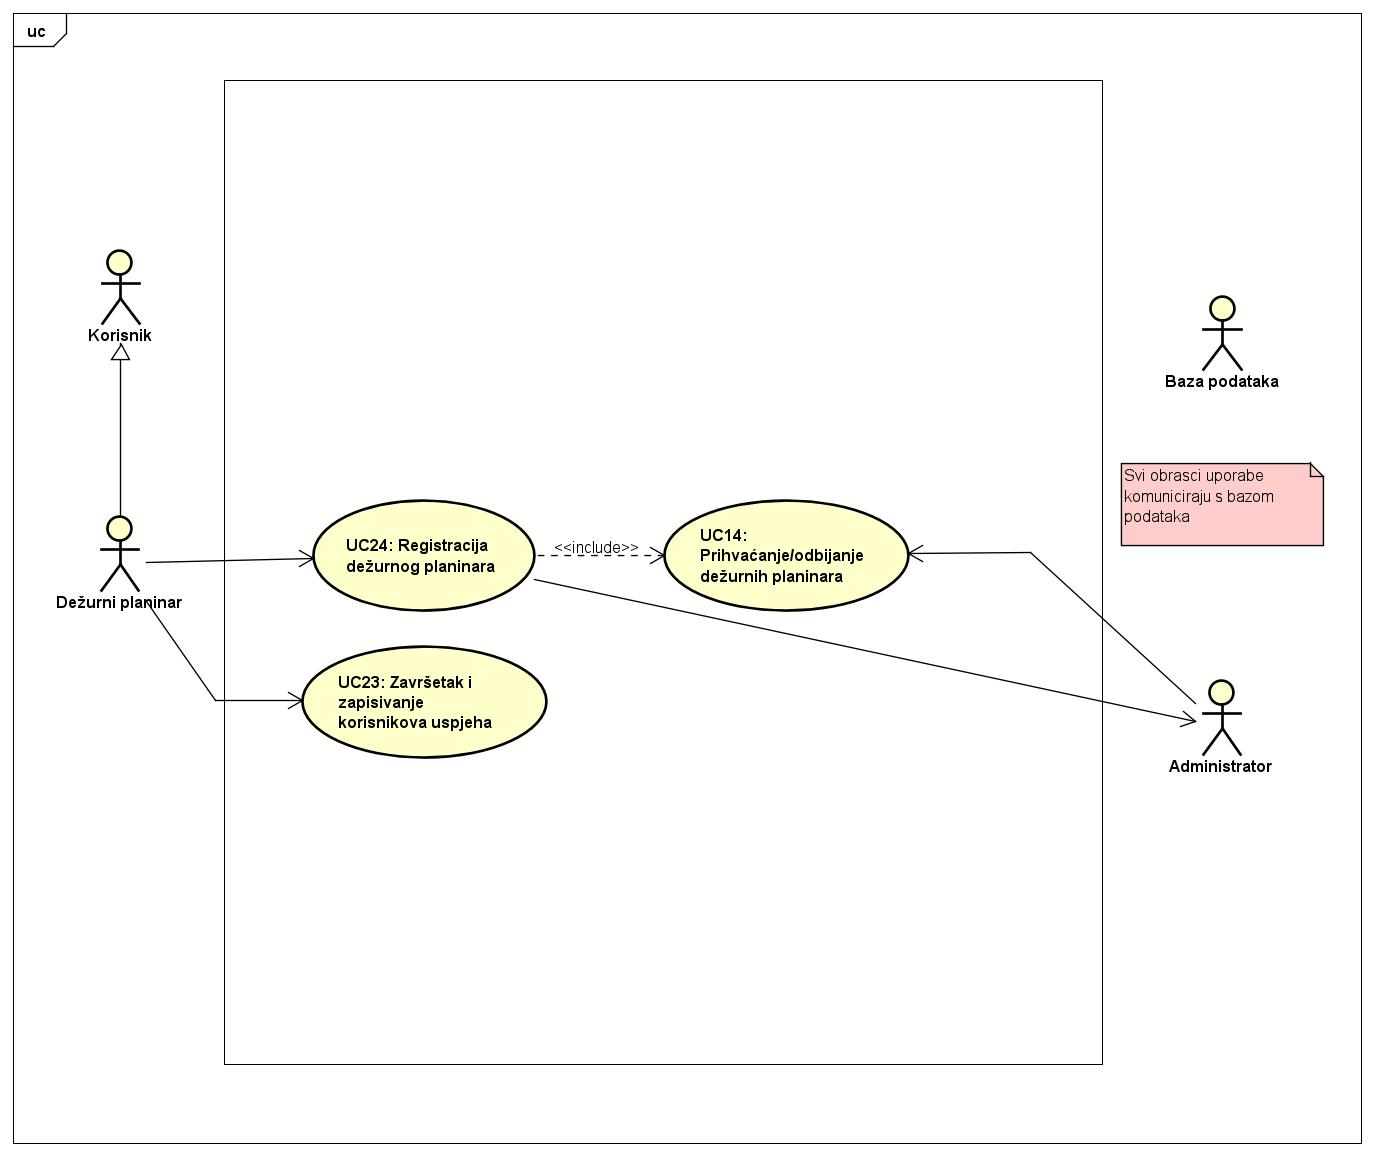
\includegraphics[width=0.9\textwidth]{slike/UC-Dezurni_planinar.jpg}
				\caption{Dijagram obrasca uporabe, funkcionalnosti  dežurnog planinara}
				\label{fig:mesh2}
			\end{figure}
			
			\begin{figure}[H]
				\centering
				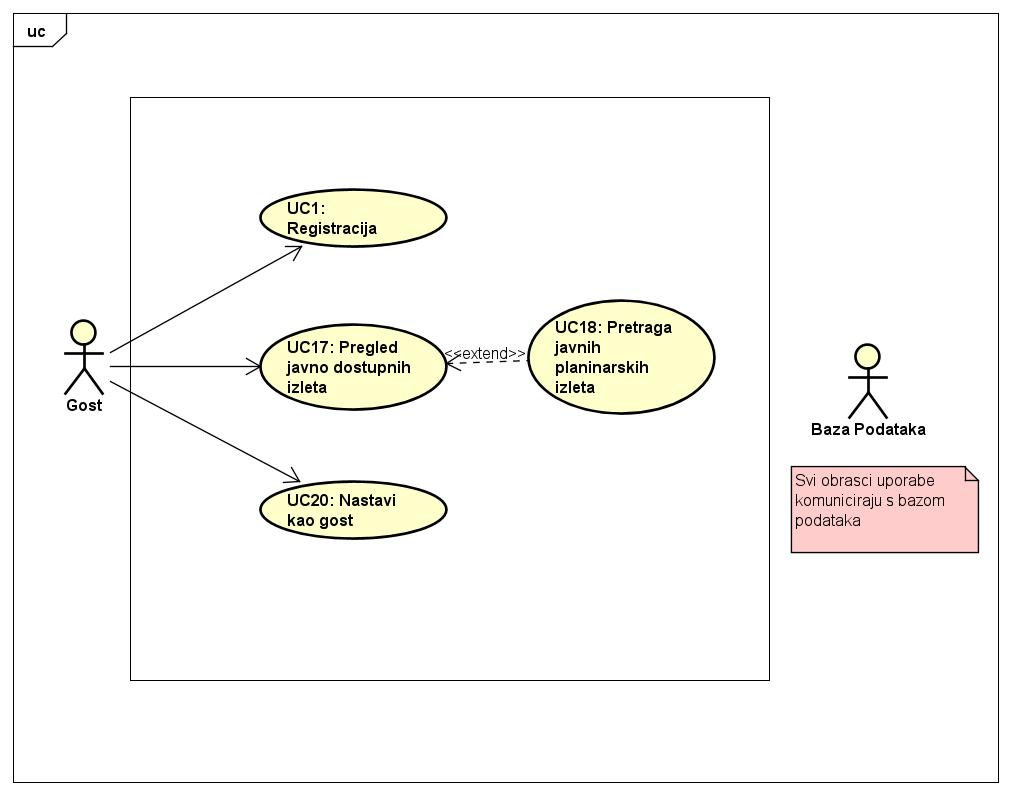
\includegraphics[width=0.9\textwidth]{slike/UC-Gost.jpg}
				\caption{Dijagram obrasca uporabe, funkcionalnosti gosta}
				\label{fig:mesh3}
			\end{figure}
		
			\begin{figure}[H]
				\centering
				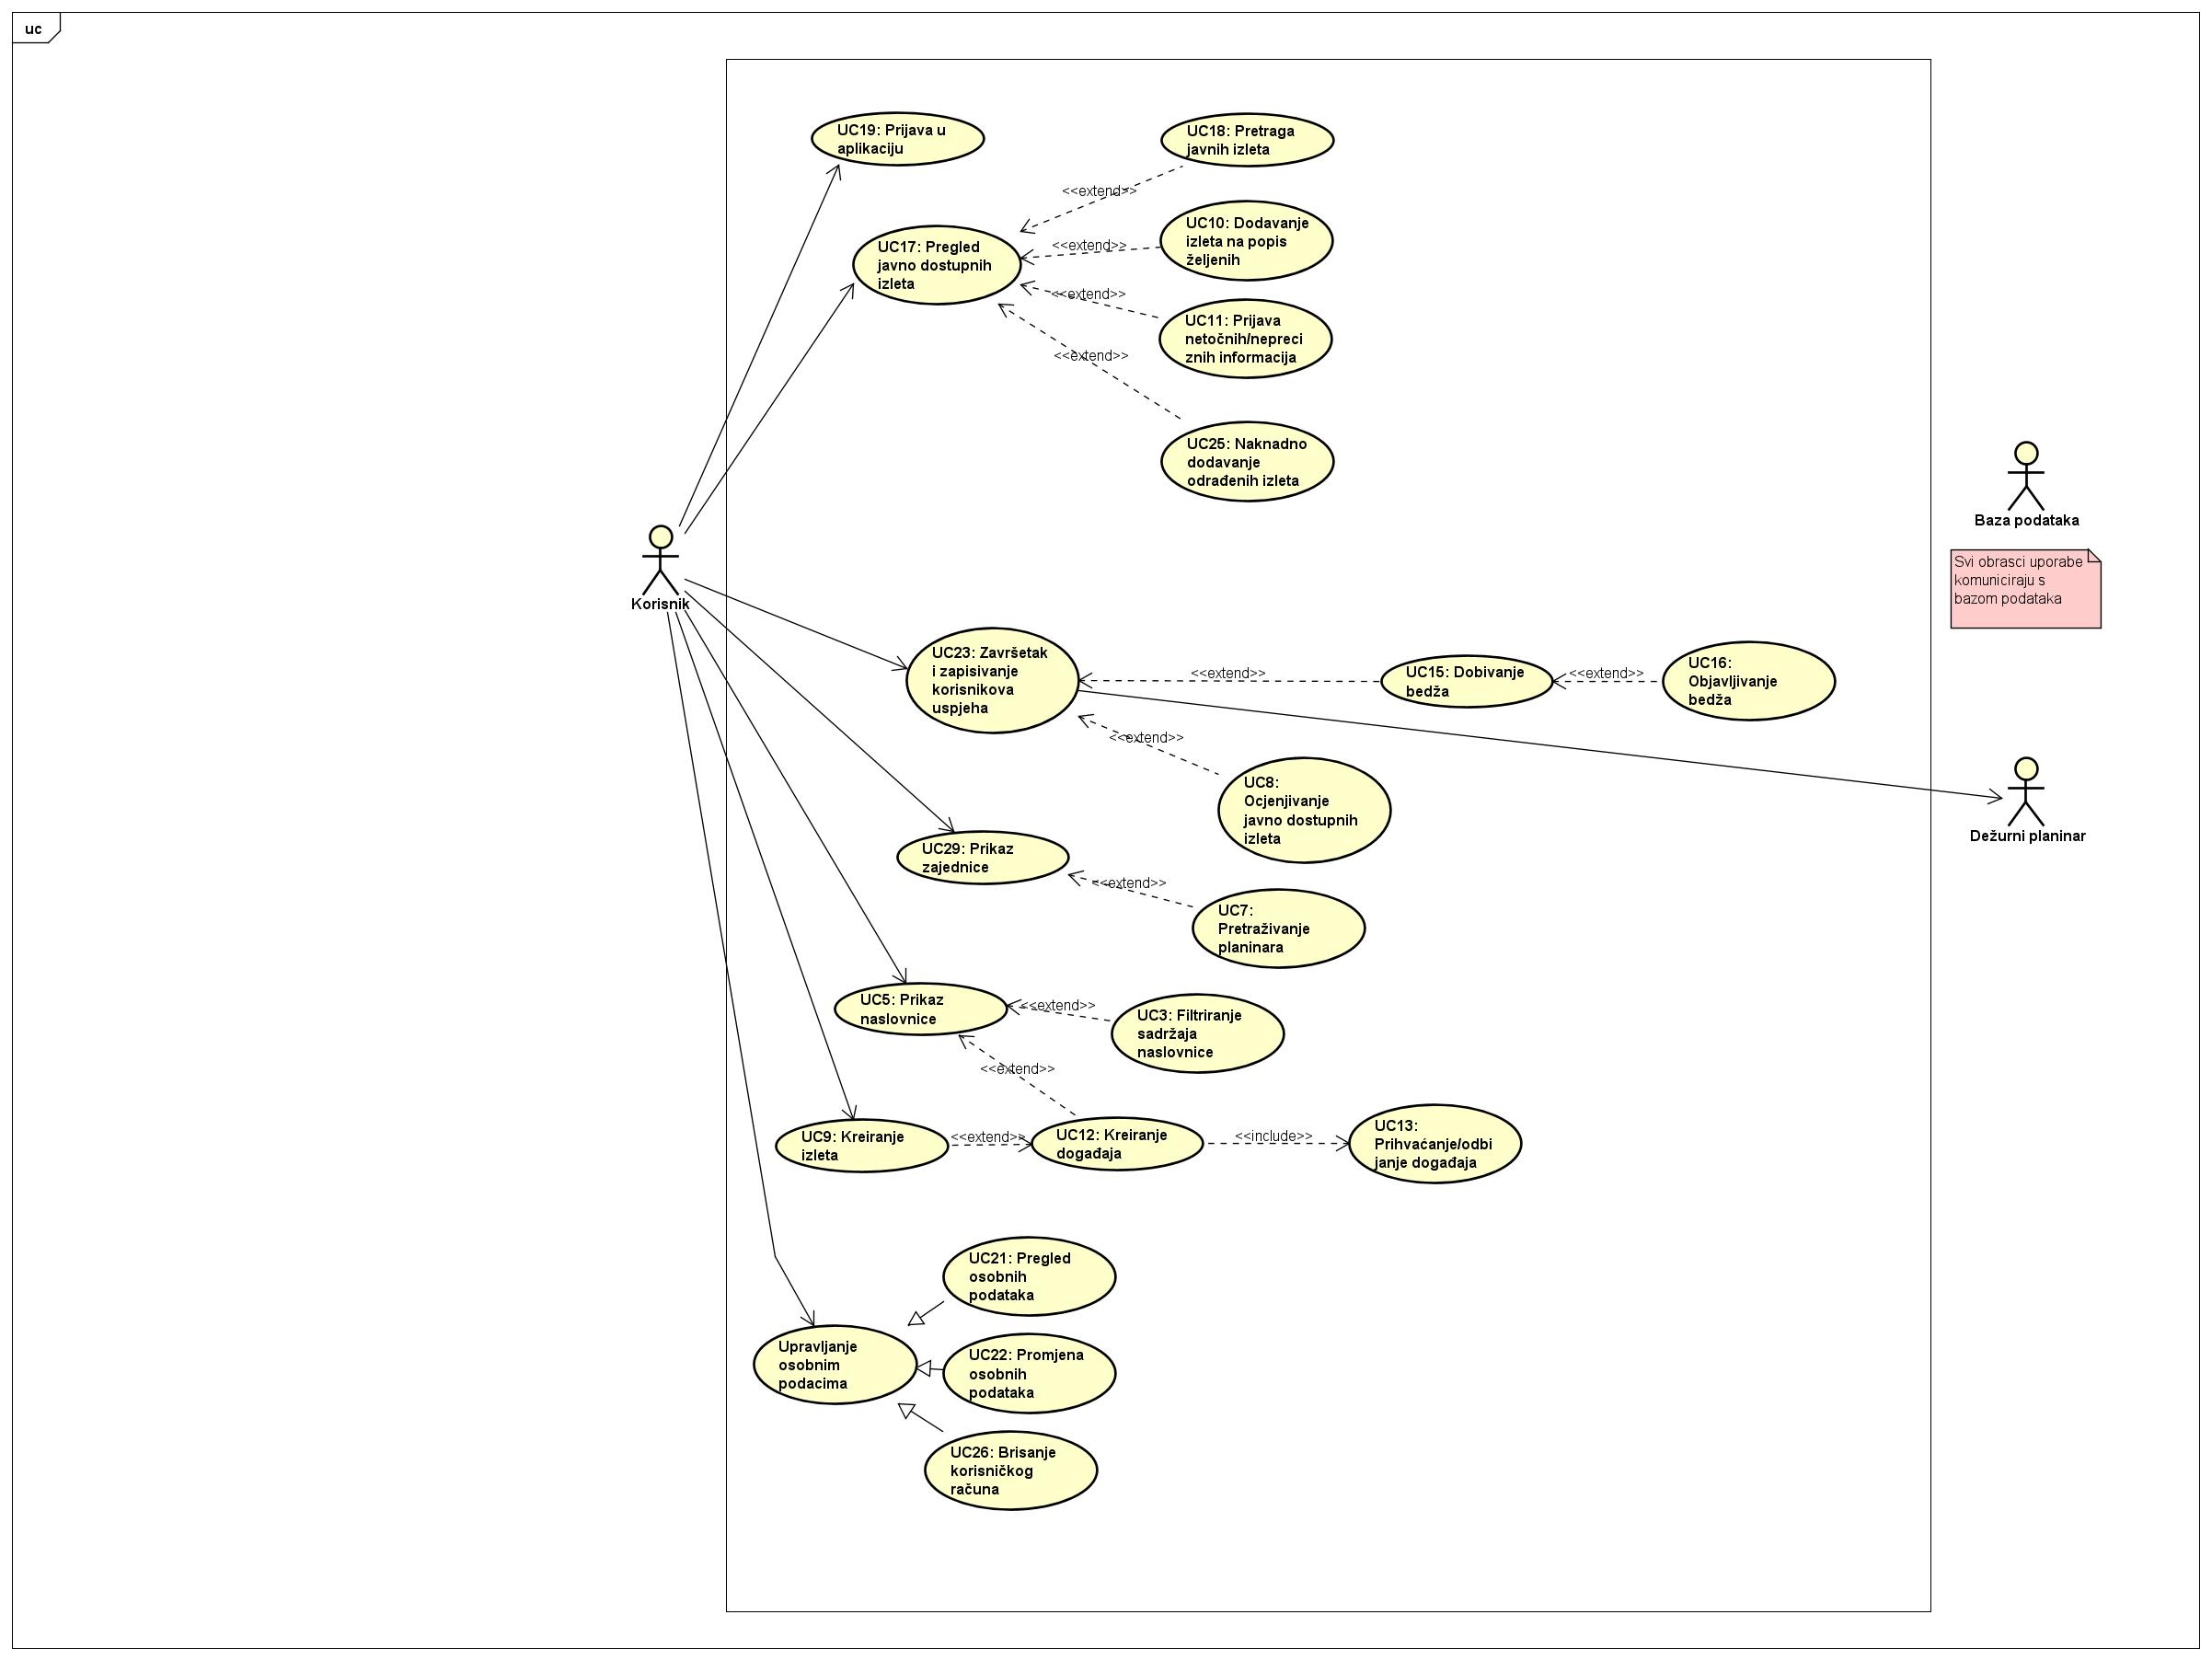
\includegraphics[width=0.9\textwidth]{slike/UC-Korisnik.jpg}
				\caption{Dijagram obrasca uporabe, funkcionalnosti korisnika}
				\label{fig:mesh4}
			\end{figure}
\newpage
	
	
		\subsection{Sekvencijski dijagrami}
		
				\textbf{ Obrazac uporabe 09 - Kreiranje izleta}\\
		
Korisnik je prijavljen i nalazi se na naslovnici ili pregledava izlete ili kreira novi događaj. Korisnik odabire opciju kreiranja izleta. Aplikacija planinarskog dnevnika šalje zahtjev bazi podataka za predložak za kreiranje novog izleta. Baza podataka vraća predložak te aplikacija korisniku prikazuje predložak. Korisnik unosi podatke novog izleta. Korisnik odabire ili kreiranje novog izleta gdje se baza ažurira, vraća potvrdu o uspjehu aplikaciji te aplikacija prikazuje uspjeh korisniku ili odabire opciju za odustajanje od kreiranja izleta te je vraćen na prethodnu stranicu.

		
		
		
				\begin{figure}[H]
					\centering
						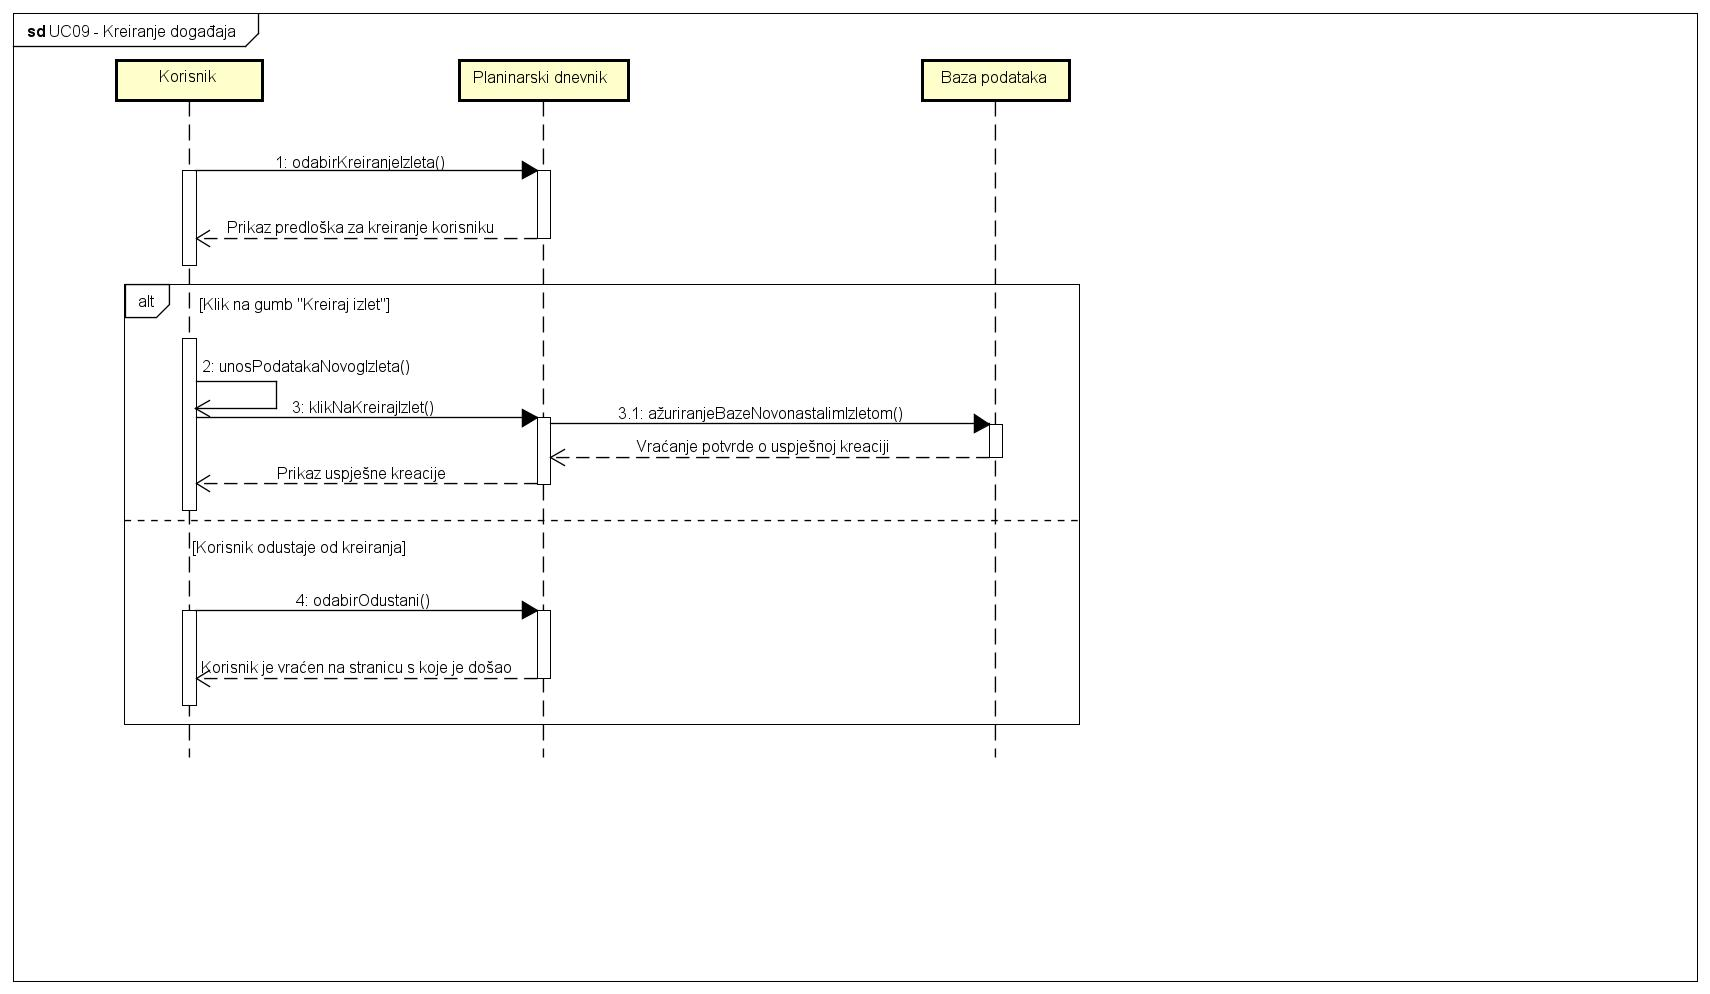
\includegraphics[width=0.9\textwidth]{slike/UC09-Kreiranje_izleta.jpg}
					\caption{Sekvencijski dijagram za UC09}
						\label{fig:mesh5}
				\end{figure}
				
\newpage
			
				\textbf{ Obrazac uporabe 18 - Pretraživanje javnih izleta}\\
				
Korisnik odabire karticu "Planinarski izleti". Planinarski dnevnik prikazuje karticu korisniku. Korisnik odabire opciju pretraživanja javnih planinarski izleta. Web-aplikacija vraća predložak za pretraživanje. Korisnik unosi podatke te klikne na gumb za pretraživanje. Web-aplikacija šalje zahtjev bazi za ispis svih planinarskih izleta koji odgovaraju kriteriju korisnika. Web-aplikacija prikazuje sve planinarske izlete koji odgovaraju korisnikovom kriteriju. Ako se korisniku ne prikazuje nijedan izlet, ponovno unosi podatke i pretražuje ili odustaje od pretrage te je vraćen na karticu "Planinarski izleti".
				
				
				
				\begin{figure}[H]
					\centering
					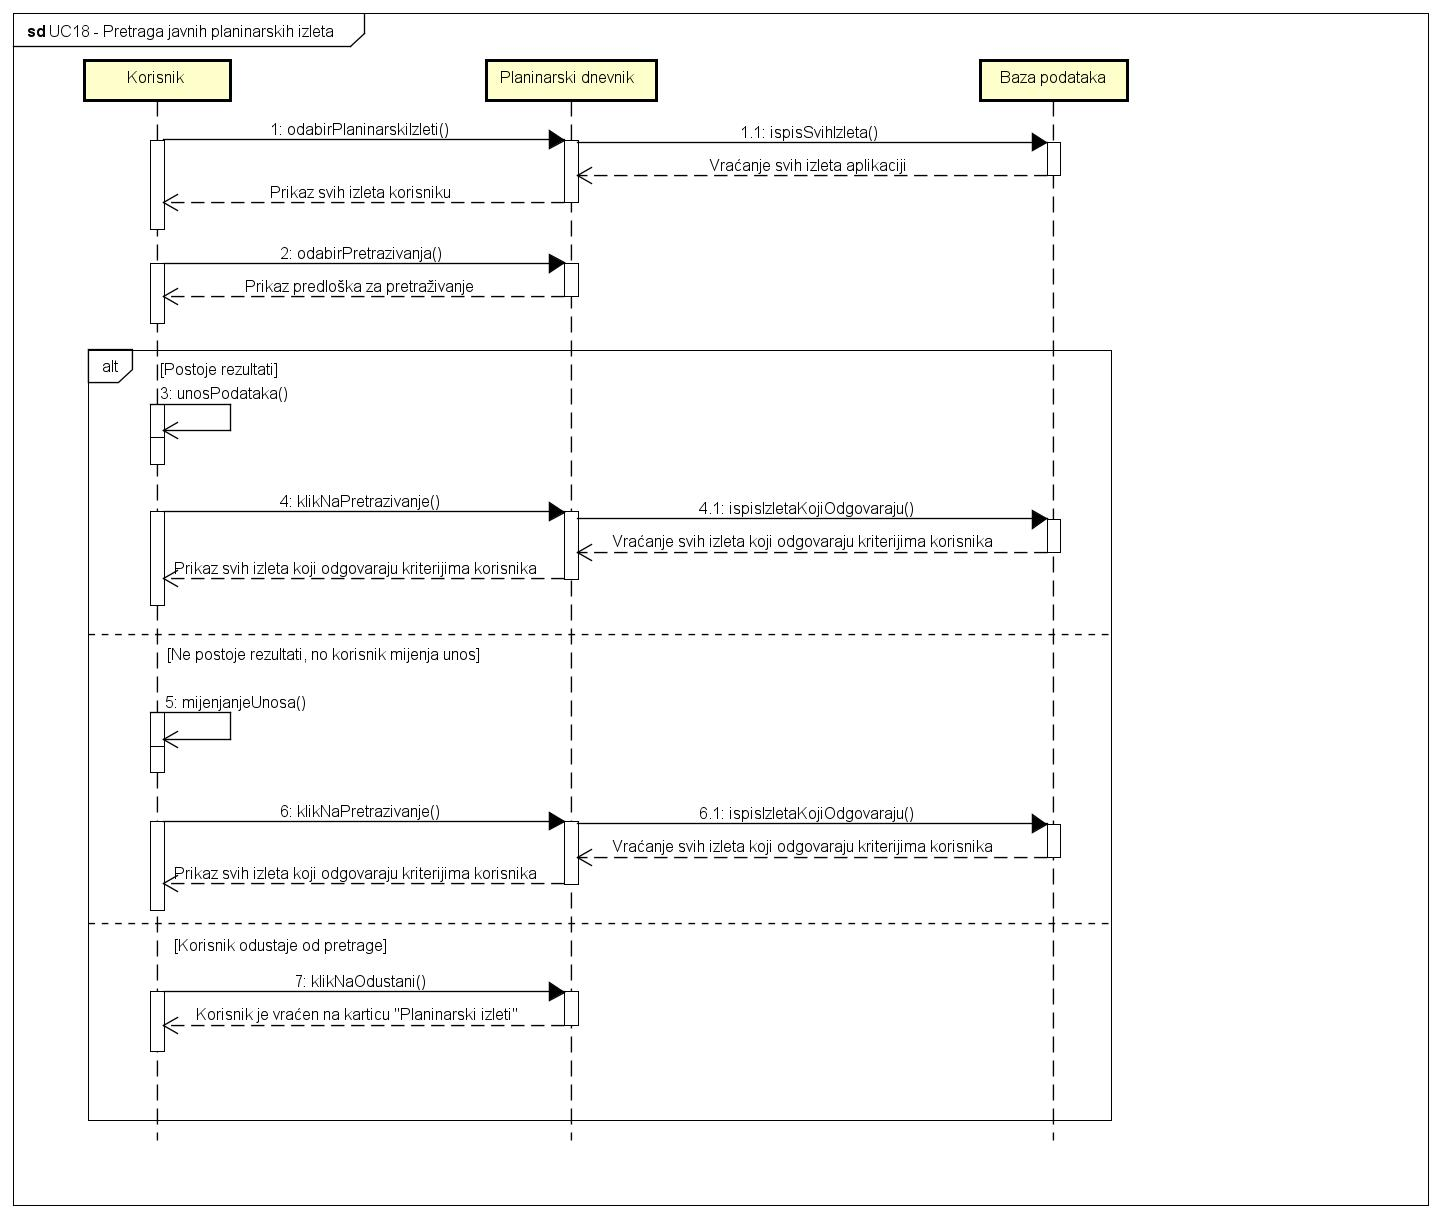
\includegraphics[width=0.9\textwidth]{slike/UC18-Pretraga_javnih_izleta.jpg}
					\caption{Sekvencijski dijagram za UC18}
					\label{fig:mesh6}
				\end{figure}

\newpage
				
				\textbf{ Obrazac uporabe 19 - Prijava u aplikaciju}\\
				
Korisnik se nalazi na stranici za prijavu i unosi svoje podatke za prijavu. Korisnik pritišće gumb za prijavu i šalje podatke koje baza zaprima te provjerava njihovu točnost. Zatim baza podataka daje povratnu informaciju o točnosti podataka nakon čega je korisnik ili prijavljen u aplikaciju (podatci su ispravni) ili je ponovno vraćen na stranicu za prijavu uz prikladnu obavijest (podatci su neispravni).
				
				
				\begin{figure}[H]
					\centering
						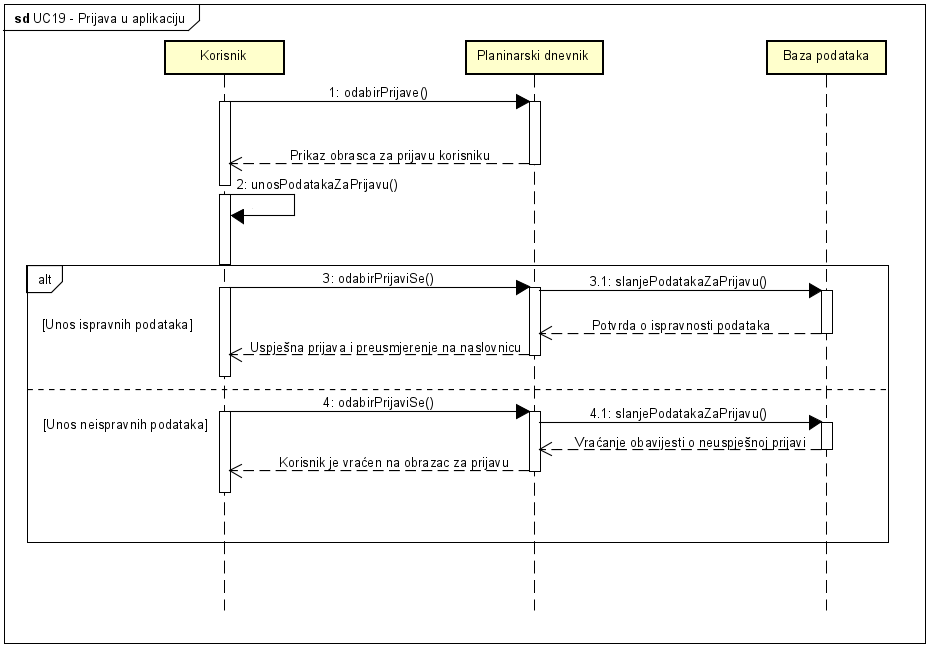
\includegraphics[width=0.9\textwidth]{slike/UC19-Prijava_u_aplikaciju.png}
					\caption{Sekvencijski dijagram za UC19}
						\label{fig:mesh7}
				\end{figure}
				
\newpage
				
				\textbf{ Obrazac uporabe 22 - Promjena osobnih podataka}\\
				
Korisnik je registriran i prijavljen u aplikaciju planinarskog dnevnika te odabire opciju ''osobni podatci''. Baza podataka prikuplja potrebne informacije o korisniku te ih šalje aplikaciji. Korisniku se prikazuju njegovi podatci te mu se pruža mogućnost da ih promijeni. Korisnik može unijeti promjene koje će baza podataka primiti i ažurirati ih te prikazati novo stanje u aplikaciji. Ukoliko korisnik unese nedozvoljene podatke aplikacija ga obavještava te je vraćen na prijašnju stranicu i može vidjeti koji podatci se nisu uspješno ažurirali.				
				
				
				\begin{figure}[H]
					\centering
						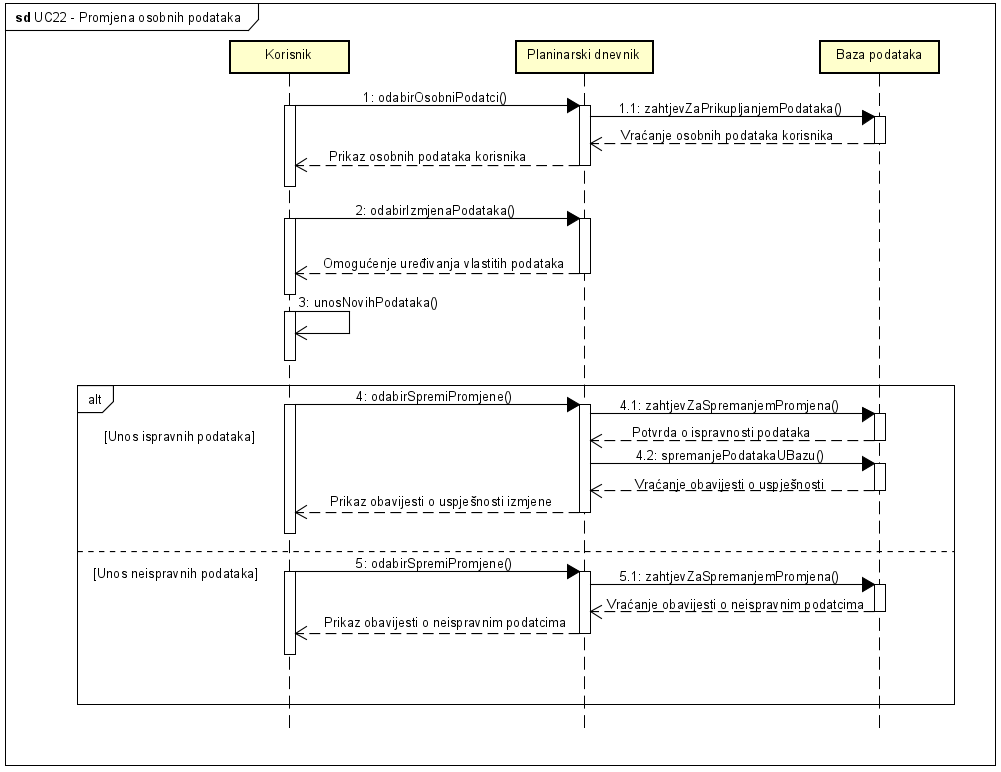
\includegraphics[width=0.9\textwidth]{slike/UC22-Promjena_osobnih_podataka.png}
					\caption{Sekvencijski dijagram za UC22}
						\label{fig:mesh8}
				\end{figure}
	
\newpage
	
\section{Ostali zahtjevi}
\begin{itemize}
	\item Sustav treba omogućiti rad više korisnika u stvarnom vremenu
	\item Korisničko sučelje i sustav moraju podržavati hrvatsku abecedu (dijakritičke znakove) pri unosu i prikazu tekstualnog sadržaja
	\item Izvršavanje dijela programa u kojem se pristupa bazi podataka ne smije trajati duže od nekoliko sekundi
	\item Sustav treba biti implementiran kao web aplikacija koristeći objektno orijentirane jezike
	\item Neispravno korištenje korisničkog sučelja ne smije narušiti funkcionalnost i rad sustava
	\item Sustav treba biti jednostavan za korištenje, korisnici se moraju znati koristiti sučeljem bez opširnih uputa
	\item Nadogradnja sustava ne smije narušavati postojeće funkcionalnosti sustava
	\item Veza s bazom podataka mora biti kvalitetno zaštićena, brza i otporna na vanjske greške 
	\item Dizajn sustava mora biti responzivan, to jest potrebno je omogućiti funkcionalno korištenje na računalu, kao i na tabletu i mobitelu
	\item Pristup sustavu mora biti omogućen iz javne mreže pomoću HTTPS
\end{itemize}